% CS631 Advanced Programming in the UNIX Environment
% Author: Jan Schaumann <jschauma@netmeister.org>
% $Id: slides.tex,v 1.2 2005/11/01 16:41:35 jschauma Exp $
\special{! TeXDict begin /landplus90{true}store end }

\documentclass[xga]{xdvislides}
\usepackage[landscape]{geometry}
\usepackage{graphics}
\usepackage{graphicx}
\usepackage{colordvi}
\usepackage{xcolor}

\begin{document}
\setfontphv

%%% Headers and footers
\lhead{\slidetitle}
\chead{CS631 - Advanced Programming in the UNIX Environment}
\rhead{Slide \thepage}
\lfoot{\Gray{Lecture 11: Shared Libraries }}
\cfoot{\relax}
\rfoot{\Gray{\today}}

\newcommand{\smallish}{\fontsize{15}{20}\selectfont}

\vspace*{\fill}
\begin{center}
	\Hugesize
		CS631 - Advanced Programming in the UNIX Environment\\
		-- \\
		Shared Libraries\\
	\hspace*{5mm}\blueline\\ [1em]
	\Normalsize
		Department of Computer Science\\
		Stevens Institute of Technology\\
		Jan Schaumann\\
		\verb+jschauma@stevens.edu+\\
		\verb+https://www.cs.stevens.edu/~jschauma/631/+
\end{center}
\vspace*{\fill}

\subsection{Shared Libraries}
\begin{verbatim}
#include <openssl/rand.h>
int main(int argc, char **argv) {
        int i; unsigned char data[NUM];

        if (RAND_bytes(data, NUM) == 0)
                err(EXIT_FAILURE, "Unable to generate random data: %s\n",
                                strerror(errno));
        for (i=0; i<NUM; i++)
                printf("%02X", data[i]);
        printf("\n");
        exit(EXIT_SUCCESS);
}
$ cc -Wall -c rand.c
$ cc -Wall rand.o
rand.o: In function `main':
rand.c:(.text+0x1c): undefined reference to `RAND_bytes'
$ cc -Wall rand.o -lcrypto
\end{verbatim}

\subsection{Shared Libraries}
What is a shared library, anyway?
\begin{itemize}
	\item contains a set of callable C functions (i.e., implementation
		of function prototypes defined in {\tt .h} header files)
	\item code is position-independent (i.e., code can be executed anywhere
		in memory)
	\item shared libraries can be loaded/unloaded at execution time or at will
	\item libraries may be {\em static} or {\em dynamic}
\end{itemize}

\subsection{Shared Libraries}
What is a shared library, anyway?
\begin{itemize}
	\item contains a set of callable C functions (i.e., implementation
		of function prototypes defined in {\tt .h} header files)
	\item code is position-independent (i.e., code can be executed anywhere
		in memory)
	\item shared libraries can be loaded/unloaded at execution time or at will
	\item libraries may be {\em static} or {\em dynamic}
\end{itemize}
\begin{verbatim}
$ man 3 fprintf
$ grep " fprintf" /usr/include/stdio.h
\end{verbatim}


\subsection{Shared Libraries}
How do shared libraries work?
\begin{itemize}
	\item contents of {\em static} libraries are pulled into the
		executable at link time
	\item contents of {\em dynamic} libraries are used to resolve
		symbols at {\bf link time}, but loaded at {\bf execution time} by the
		{\em dynamic linker}
	\item contents of {\em dynamic} libraries may be loaded at {\bf any
		time} via explicit calls to the dynamic linking loader interface
		functions
\end{itemize}

\subsection{Executable and Linkable Format}

{\bf ELF} is a file format for executables, object code, shared libraries
etc.

\begin{center}
	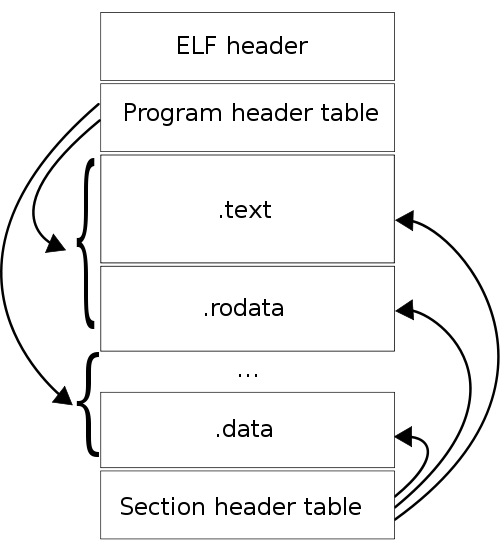
\includegraphics[scale=0.5]{pics/elf.eps}
\end{center}
More details:
\verb+http://www.cs.stevens.edu/~jschauma/631/elf.html+

\verb+http://www.thegeekstuff.com/2012/07/elf-object-file-format/+
\Normalsize


\subsection{Executable and Linkable Format}

{\bf ELF} is a file format for executables, object code, shared libraries

\begin{itemize}
	\item {\em relocatable file} -- can be linked
		together with others to produce a
		shared library or an executable (e.g. \verb+foo.o+)
	\item {\em shared object file} -- position
		independent code; used by the dynamic
		linker to create a process image (e.g. \verb+libfoo.so+)
	\item {\em executable} -- just what it sounds like (e.g. \verb+a.out+)
\end{itemize}

\subsection{Executable and Linkable Format}
\begin{verbatim}
$ cc -Wall -c main.c
$ hexdump -C main.o | head -2
\end{verbatim}
\ttfamily
00000000  \textcolor{red}{7f 45 4c 46} \textcolor{green}{02} 01 01 \textcolor{orange}{00}  00 00 00 00 00 00 00 00
00000010  \textcolor{blue}{01 00} \textcolor{purple}{3e 00} 01 00 00 00  00 00 00 00 00 00 00 00
\begin{verbatim}

$ file main.o
\end{verbatim}
main.o: \textcolor{red}{ELF} \textcolor{green}{64-bit} \textcolor{blue}{LSB relocatable}, \textcolor{purple}{x86-64}, \textcolor{orange}{version 1 (SYSV)}, not stripped
\setfontphv

\subsection{Executable and Linkable Format}
\begin{verbatim}
$ hexdump -C /lib/libc.so | head -2
\end{verbatim}
\ttfamily
00000000  \textcolor{red}{7f 45 4c 46} \textcolor{green}{02} \textcolor{magenta}{01} \textcolor{gray}{01} \textcolor{orange}{00} \textcolor{brown}{00} 00 00 00 00 00 00 00 \\
00000010  \textcolor{blue}{03 00} \textcolor{purple}{3e 00} \textcolor{yellow}{01 00 00 00}  \textcolor{olive}{70 b7 03} 00 00 00 00 00
\begin{verbatim}
$ readelf -h /lib/libc.so
ELF Header:
\end{verbatim}
\begin{tabular}{ll}
Magic: & \textcolor{red}{7f 45 4c 46} \textcolor{green}{02} \textcolor{magenta}{01} \textcolor{gray}{01} \textcolor{orange}{00} \textcolor{brown}{00} 00 00 00 00 00 00 00 \\
Class: & \textcolor{red}{ELF}\textcolor{green}{64}\space \\
Data: & \textcolor{magenta}{2's complement, little endian} \\
Version: & \textcolor{gray}{1 (current)} \\
OS/ABI: & \textcolor{orange}{UNIX - System V} \\
ABI Version: & \textcolor{brown}{0} \\
Type: & \textcolor{blue}{DYN (Shared object file)} \\
Machine: & \textcolor{purple}{Advanced Micro Devices X86-64} \\
Version: & \textcolor{yellow}{0x1} \\
Entry point address: & \textcolor{olive}{0x3b770} \\
  ... & \\
\end{tabular}
\setfontphv

\subsection{Executable and Linkable Format}
\begin{verbatim}
$ hexdump -C a.out | head -2
\end{verbatim}
\ttfamily
00000000  \textcolor{red}{7f 45 4c 46} \textcolor{green}{02} \textcolor{magenta}{01} \textcolor{gray}{01} \textcolor{orange}{00} \textcolor{brown}{00} 00 00 00 00 00 00 00 \\
00000010  \textcolor{blue}{02 00} \textcolor{purple}{3e 00} \textcolor{yellow}{01 00 00 00}  \textcolor{olive}{e0 07 40} 00 00 00 00 00
\begin{verbatim}
$ readelf -h a.out
ELF Header:
\end{verbatim}
\begin{tabular}{ll}
  Magic: & \textcolor{red}{7f 45 4c 46} \textcolor{green}{02} \textcolor{magenta}{01} \textcolor{gray}{01} \textcolor{orange}{00} \textcolor{brown}{00} 00 00 00 00 00 00 00 \\
  Class: & \textcolor{red}{ELF}\textcolor{green}{64} \\
  Data: & \textcolor{magenta}{2's complement, little endian} \\
  Version: & \textcolor{gray}{1 (current)} \\
  OS/ABI: & \textcolor{orange}{UNIX - System V} \\
  ABI Version: & \textcolor{brown}{0} \\
  Type: & \textcolor{blue}{EXEC (Executable file)} \\
  Machine: & \textcolor{purple}{Advanced Micro Devices X86-64} \\
  Version: & \textcolor{yellow}{0x1} \\
  Entry point address: & \textcolor{olive}{0x4007e0} \\
  ... \\
\end{tabular}
\setfontphv


\subsection{Understanding object files}
\begin{verbatim}
$ cc -Wall ldtest1.c ldtest2.c main.c
$ nm a.out
                 U _libc_init
00000000004007a0 T _start
                 U atexit
0000000000600ea0 B environ
                 U exit
0000000000400990 T ldtest1
00000000004009b4 T ldtest2
00000000004009d8 T main
                 U printf
$ ldd a.out
a.out:
        -lgcc_s.1 => /usr/lib/libgcc_s.so.1
        -lc.12 => /usr/lib/libc.so.12
\end{verbatim}
See also: \verb+objdump -x a.out+

\subsection{Statically Linked Shared Libraries}
Static libraries:
\begin{itemize}
	\item created by {\tt ar(1)}
	\item usually end in {\tt .a}
	\item contain a symbol table within the archive (see {\tt
		ranlib(1)})
\end{itemize}

\subsection{Statically Linked Shared Libraries}
\begin{verbatim}
$ cc -Wall -c ldtest1.c
$ cc -Wall -c ldtest2.c
$ cc -Wall main.c
[...]
$ cc -Wall main.c ldtest1.o ldtest2.o
$
\end{verbatim}

\subsection{Statically Linked Shared Libraries}
\begin{verbatim}
$ cc -Wall -c ldtest1.c ldtest2.c
$ ar -vq libldtest.a ldtest1.o ldtest2.o
$ ar -t libldtest.a
$ nm libldtest.a

ldtest1.o:
0000000000000000 T ldtest1
                 U printf

ldtest2.o:
0000000000000000 T ldtest2
                 U printf
$ objdump -x libldtest.a
\end{verbatim}

\subsection{Statically Linked Shared Libraries}
\begin{verbatim}
$ cc -Wall main.c libldtest.a
$ mv libldtest.a /tmp/
$ ./a.out

$ cc -Wall main.c -L/tmp -lldtest -o a.out.dyn
$ cc -static main.o -L/tmp -lldtest -o a.out.static
$ ls -l a.out.*
$ ldd a.out.*
$ nm a.out.dyn | wc -l
$ nm a.out.static | wc -l
\end{verbatim}

\subsection{Dynamically Linked Shared Libraries}
Dynamic libraries:
\begin{itemize}
	\item created by the compiler/linker (i.e. multiple steps)
	\item usually end in {\tt .so}
	\item frequently have multiple levels of symlinks providing
		backwards compatibility / ABI definitions
\end{itemize}

\subsection{Dynamically Linked Shared Libraries}
\begin{verbatim}
$ cc -Wall -c -fPIC ldtest1.c ldtest2.c
$ mkdir lib
$ cc -shared -Wl,-soname,libldtest.so.1 -o lib/libldtest.so.1.0 ldtest1.o ldtest2.o
$ ln -s libldtest.so.1.0 lib/libldtest.so.1
$ ln -s libldtest.so.1.0 lib/libldtest.so
$ cc -static -Wall main.o -L./lib -lldtest
ld: cannot find -lldtest
$ mv /tmp/libldtest.a lib
$ cc -static -Wall main.o -L./lib -lldtest
$ ./a.out
[...]
$ cc -Wall main.o -L./lib -lldtest
$ ./a.out
[...]
$ ldd a.out
[...]
\end{verbatim}

\subsection{Dynamically Linked Shared Libraries}
Wait, what?
\begin{verbatim}
$ export LD_LIBRARY_PATH=${LD_LIBRARY_PATH}:./lib
$ ldd a.out
[...]
$ ./a.out
[...]
$ mkdir lib2
$ cc -Wall -c -fPIC ldtest1.2.c
$ cc -shared -Wl,-soname,libldtest.so.1 -o lib2/libldtest.so.1.0 ldtest1.2.o ldtest2.o
$ ln -s libldtest.so.1.0 lib2/libldtest.so.1
$ ln -s libldtest.so.1.0 lib2/libldtest.so
$ export LD_LIBRARY_PATH=./lib2:$LD_LIBRARY_PATH
$ ldd a.out  # note: no recompiling!
[...]
$ ./a.out
[...]
\end{verbatim}

\subsection{Dynamically Linked Shared Libraries}
Avoiding {\tt LD\_LIBRARY\_PATH}:
\begin{verbatim}
$ cc -Wall main.o -L./lib -lldtest -Wl,-rpath,./lib
$ echo $LD_LIBRARY_PATH
[...]
$ ldd a.out
[...]
$ ./a.out
[...]
$ unset LD_LIBRARY_PATH
$ ldd a.out
[...]
$ ./a.out
[...]
$
\end{verbatim}

\subsection{Dynamically Linked Shared Libraries}
But:
\begin{verbatim}
$ cc -Wall -fPIC -c evil.c
$ cc -shared -Wl,-soname,libldtest.so.1 -o lib3/libldtest.so.1.0 \
        ldtest1.o ldtest2.o evil.o
$ export LD_PRELOAD=./lib3/libldtest.so.1.0
$ ldd a.out
[...]
$ ./a.out 2>/dev/null
[...]
$
\end{verbatim}

\subsection{Dynamically Linked Shared Libraries}
\begin{verbatim}
$ export LD_DEBUG=help # glibc>=2.1 only
$ ./a.out
[...]
$ LD_DEBUG=all ./a.out
[...]
\end{verbatim}

\subsection{Dynamically Linked Shared Libraries}
Explicit loading of shared libraries:
\begin{itemize}
	\item {\tt dlopen(3)} creates a handle for the given library
	\item {\tt dlsym(3)} returns the address of the given symbol
\end{itemize}

\begin{verbatim}
$ cc -Wall rand.c -lcrypto
$ cc -Wall -rdynamic dlopenex.c
$ ./a.out
\end{verbatim}

\subsection{Homework}
\verb+https://www.cs.stevens.edu/~jschauma/631/f17-hw4.html+ \\

\begin{verbatim}
$ cat hello.c
#include <greet.h>
#include <stdio.h>

int main(void) {
        greet();
        if (setgreeting("Howdy!") != 0) {
                fprintf(stderr, "Unable to set greeting!\n");
        }
        greet();
        hello("you there", getgreeting());
        return 0;
}
$ cc -Wall hello.c -I./libgreet -L./libgreet -Wl,-rpath,./libgreet -lgreet
\end{verbatim}

\subsection{Reading}
\begin{itemize}
	\item \verb+https://www.bell-labs.com/usr/dmr/www/man51.pdf+
	\item \verb+https://en.wikipedia.org/wiki/Executable_and_Linkable_Format+
	\item \verb+https://www.cs.stevens.edu/~jschauma/631/elf.html+
	\item \verb+http://www.thegeekstuff.com/2012/07/elf-object-file-format/+
	\item \verb+https://is.gd/XPn9Ul+
\end{itemize}


\end{document}
